\documentclass{article}

\usepackage[spanish]{babel}
\usepackage[numbers,sort&compress]{natbib}
\usepackage[T1]{fontenc}
\usepackage[ansinew]{inputenc}
\usepackage{graphicx}
\usepackage{url}
\usepackage[numbers,sort&compress]{natbib}

\title { Movimiento Browniano}
\author{Anahi Llano}

\begin{document}

\maketitle

\section{Introducci\'on}\label{intro}

El movimiento browniano es un movimiento que ocurre de manera aleatoria observable en part\'iculas microsc\'opicas que se encuentran en un medio fluido, como es el polen en una gota de agua. Tal movimiento recibe su nombre en honor al biol\'ogo bot\'anico Robert Brown, quien en 1827 observo como es que las part\'iculas de polen se despazaban de manera aleatoria sin alguna raz\'on. El movimiento aleatorio de estas part\'iculas se debe a que su superficie es bombardeada incesantemente por las mol\'eculas, es decir, los \'atomos del fluido sometidas a una agitaci\'on t\'ermica. \citet{baz}
A pesar de que fue Robert Brown el primero el observar este fen\'omeno, el primero en explicarlo fue Einstein en 1905.
Cuando se realiza una simulaci\'on del movimiento browniano este se representa en movimientos trat\'andose de una caminata, en donde la part\'icula parte desde un origen y esta da "pasos" discretos (tiempo) de forma aleatoria, realizado desde una dimensi\'on hasta las que podamos imaginar trat\'andose de un modelo matem\'atico. \citep{Eli}. Con estos estudios es posible predecir las tendencias del comportamiento de las part\'iculas de acuerdo con las diferentes variables que sean tomadas en cuenta.

\section{Objetivo}\label{objec}

Observar  los efectos de la dimensi\'on en el tiempo de regreso al origen del movimiento Browniano para dimensiones 1 a 8 en incrementos lineales de uno, variando el n\'umero de pasos de la caminata como potencias de dos con exponente de 5 a 10 en incrementos lineales de uno, con 50 repeticiones del experimento para cada combinaci\'on

\newpage
\section{Metodolog\'ia}\label{met}

Se utilizo el paquete estad\'istico R en la vercion 4.0.2 para estudiar los efectos de la dimensi\'on en el tiempo de regreso al origen del movimiento Browniano.
La pr\'actica consisti\'o en simular una caminata variando las dimensiones entre 1 y 8 y tambi\'en los pasos de la misma como potencias de dos con exponente de 5 a 10 en incrementos lineales de uno.  Se realizaron 50 repeticiones para cada caso, con estos datos se
calcul\'o la probabilidad de regreso para cada una de las 8 dimensiones, as\'i mismo, se observ\'o el efecto de la dimensi\'on en el tiempo de regreso del origen de la caminata sobre el comportamiento de la part\'icula.

Los resultados obtenidos fueron graficados por medio de diagrama de caja y bigotes, en el cual se observa el efecto de la dimesi\'on en el tiempo de regreso al origen de la part\'icula en la cual se representa tal movimiento.

\section{Resultados y Discusi\'on}\label{res}

Una vez ejecutada la simulacion por medio de R, se obtuvieron una matriz de datos correspondientes a los porcentajes de regreso al punto de origen para cada dimensi\'on, as\'i como cada duraci\'on de la caminata. En el cuadro \ref{t1} se muestra el conjunto de datos con el cual se realiz\'o el an\'alisis de la presente.
Una vez obtenida la matriz de datos se construy\'o el diagrama de caja/bigote, (Figura \ref{f1} ), para observar c\'omo es que se comporta una part\'icula con movimiento browniano), en donde cada caja corresponde a una dimensi\'on donde se ven agrupados los porcentajes de regreso al punto de origen en los diferentes tiempos de la caminata.
As\'i como en la Figura \ref{f2}, se observa la distancia m\'axima que recorri\'o la part\'icula en cada dimensi\'on.

\begin{table} 
 \caption{Datos obtenidos por R.}
  \cite{tarea1},
 \label{t1}
 \begin{center}
 \begin{tabular}{rrr}
\texttt{pot} & \texttt{porc} & \texttt{dim} \\
5  &  96  &  1 \\
5  &  80  &  2 \\
5  &  32  &  3 \\
5  &  16  &  4 \\
5  &  8    &   5 \\
5  &  14  &   6 \\
5  &  4    &   7 \\
5  &  14  &   8 \\
$\vdots$ &   $\vdots$ &   $\vdots$ \\
10  &   70  &  2 \\
10  &  24   &  3 \\
10  &  14   &  4 \\
10  &   6    &  5 \\
10  &  14   &  6 \\
10  &  8     &  7 \\
10  &  8     &  8 \\
\end{tabular}
\end{center}
\end{table}


\begin{figure}
  \begin{center}
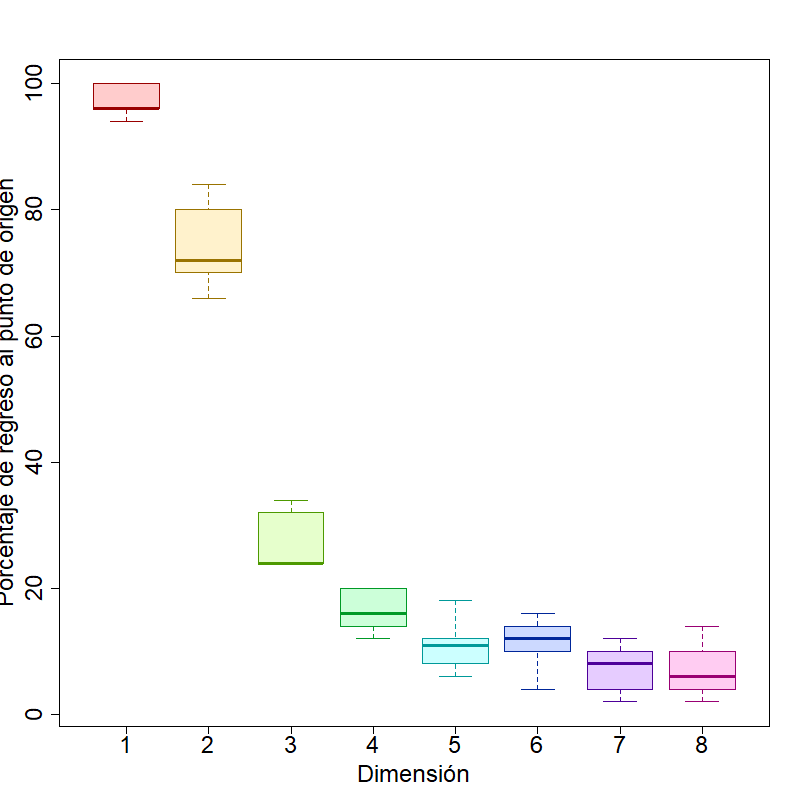
\includegraphics[scale=0.3]{pr1sim.png}
\end{center}
  \caption{Probabilidad de regreso por dimensi\'on.}
  \label{f1}
  \cite{tarea1}

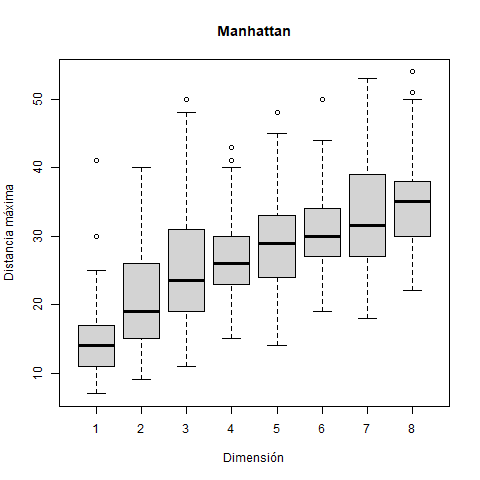
\includegraphics[scale=0.5]{p1mr.png}
 \caption{Distancia maxima.}
  \label{f2}
  \cite{tarea1}
\end{figure}

\newpage
\section{Conclusiones}\label{con}

El movimiento de una part\'icula se realiza de manera aleatoria, es posible observar tal movimiento mediante modelos matem\'aticos variando tanto, el largo de la caminata(tiempo), como la dimensi\'on en la que se encuentre, ya que este es posible observar en un modelo matem\'atico, en todas las dimensiones que se puedan ocurrir y esta siempre vuelve a su punto de origen, pero conforme vamos teniendo m\'as dimensiones es m\'as dif\'icil regresar a su origen.

\bibliography{biblio}
\bibliographystyle{plainnat}

\end{document}




